\documentclass[tikz,border=1pt]{standalone}

\usepackage{pgfplots}
% \usepgfplotslibrary{external}
% \tikzexternalize[prefix=tikz/]
\usepackage{pgfplotstable}

\usepackage{amssymb}
\usepackage{amsmath}
\usepackage{amsthm}

\pgfplotsset{compat=1.17}

\usetikzlibrary{calc,patterns,angles,quotes}    

\begin{document}

\begin{tikzpicture}
  \begin{loglogaxis} [
    title=Convergence Plot,
    xlabel={Degrees of Freedom},
    ylabel={$L_2$-Error},
    grid=major,
    legend entries={$d=2$, $d=3$, $d=4$},
    ]
    \addplot table {data_d2.dat};
    \addplot table {data_d3.dat};
    \addplot table {data_d4.dat};
    \addplot table [
    x=dof,
    y={create col/linear regression={y=l2_err,
        variance list={1000,800,600,500,400,200,100}}}] {data_d4.dat}
    coordinate [pos=0.25] (A)
    coordinate [pos=0.4] (B)
    ;

    \xdef\slope{\pgfplotstableregressiona}
    
    \draw [-stealth] (A) -| (B)
    node [pos=0.75,anchor=west]{\pgfmathprintnumber{\slope}}
    ;
  \end{loglogaxis}
\end{tikzpicture}

\begin{tikzpicture}
  \begin{loglogaxis}
    \addplot table {data_d2.dat}
    coordinate [pos=0.25] (A)
    coordinate [pos=0.4] (B)
    ;

    \draw [-stealth] (A) -| (B);

    \node [pin=0:Special.] at (769,1.623e-04) {};
  \end{loglogaxis}
\end{tikzpicture}

\begin{tikzpicture}
  \begin{axis}[
    axis lines=center,
    ]
    \addplot [
    blue,
    domain=-1:1,
    samples=51,
    ] {abs(x)};
    \addplot [
    red,
    domain=-0.5:0.3,
    samples=100,
    ] {-abs(x)};
  \end{axis}
\end{tikzpicture}

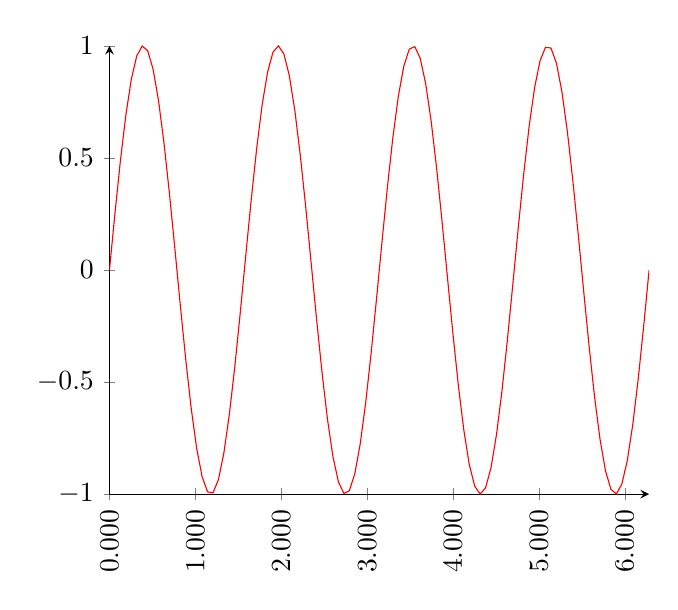
\begin{tikzpicture}
  \newcommand{\OMEGA}{4}
  \begin{axis}[
    axis lines=left,
    trig format plots=rad,
    xticklabel style={
      rotate=90,
      anchor=east,
      /pgf/number format/precision=3,
      /pgf/number format/fixed,
      /pgf/number format/fixed zerofill,
    },
    ]
  \addplot [
  red,
  domain=0:2*pi,
  samples=100,
  ] {sin(\OMEGA*x)};
  \end{axis}
\end{tikzpicture}

\begin{tikzpicture}
  \begin{axis}
  \addplot [
  red,
  domain=0:2*pi,
  samples=100,
  ] {sin(deg(x))};
  \end{axis}
\end{tikzpicture}

\begin{tikzpicture}
  \begin{axis}[
    title=My first plot,
    xlabel={$X$},
    ylabel={$Y$}
  ]
  \addplot [
  red,
  domain=-1.5:1.5,
  samples=100,
  ] {exp(-x^2)/sqrt(2*pi)};
  \end{axis}
\end{tikzpicture}


\end{document}
